\begin{figure}
    \centering
    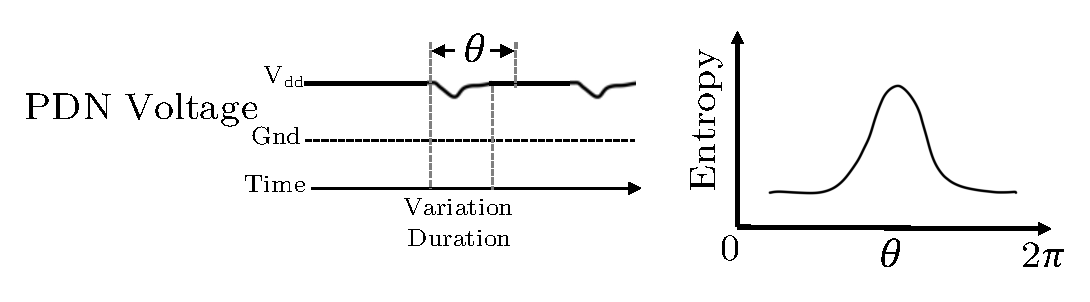
\includegraphics[width=.99\columnwidth]{img/theta-entropy.pdf}
    \caption{Demonstrating the effect of tuning $\theta$ on extracting information about a co-tenant computation. Assume that the PDN Voltage only varies for a short time, which is directly related to the execution of the target computation. If $\theta$ is too small, the sensor will not capture the entirety of the PDN variations. If $\theta$ is too large, then the sensor will capture the variations plus additional irrelevant PDN behaviors. The maximum channel capacity (in terms of entropy) is achieved when $\theta$ exactly matches the duration of the PDN variations.}
    \label{fig:theta-entropy}
    \vspace{-10pt}
\end{figure}